\begin{frame}
    \frametitle{ELPI}
    \begin{itemize}
        \item Extension of $\lambda$Prolog\com{supports higher-order abstract syntax}
        \item Generic inference/reasoning step after semantics construction
        \item Goal: Use it for semantic/pragmatic analysis
    \end{itemize}

    \begin{minipage}[t][4cm][t]{\textwidth}
        \pause
        \vspace{2em}
        Example: Discard wrong readings in controlled natural language

        \vspace{1em}
        \only<2>{
            \tikzset{every picture/.style={line width=0.7pt}}
            \begin{tikzpicture}[yscale=0.5]
                \node(str0) at (-4,0) {\str{the ball has a mass of 5kg}};
                \node(ast0) at (-0.5,0) {AST};
                \node(log0) at (4,0) {\ifcolorful\color{logicfont}\fi$\text{mass}(\text{theball}, \text{quant}(5, \text{kilo gram}))$};
                \draw[-{Straight Barb[length=6.3,width=5.0]},gray] (str0) -- (ast0);
                \draw[-{Straight Barb[length=6.3,width=5.0]},gray] (ast0) -- (log0);
            \end{tikzpicture}
        }
        \only<3>{\disablepart{crossout}}
        \only<4>{\enablepart{crossout}}
        \enablepart{switchtonmexample}
        \onslide<3-4>{
            \includestandalone[width=\textwidth]{fig/cnl-simple-discard} 
        }
    \end{minipage}


    \only<5>{
        \begin{tikzpicture}[overlay,remember picture]
            \fill[gray!80,opacity=0.8] (current page.north west) rectangle (current page.south east);
            \node at (current page.center) { 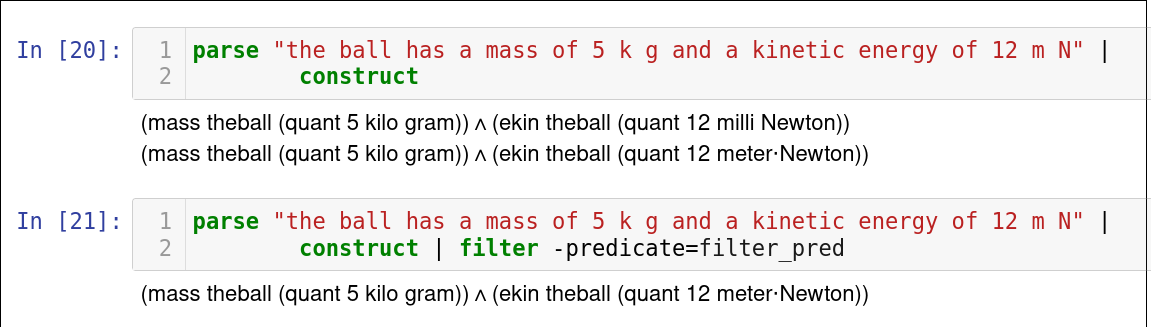
\includegraphics[width=0.85\textwidth]{img/screenshot-glif-3.png} };
        \end{tikzpicture}
    }
\end{frame}
